\documentclass{standalone}
\usepackage{tikz}
\usepackage{tkz-euclide}
\usepackage{ctex}
\pagestyle{empty}
\setCJKmainfont{Noto Serif CJK SC}
\usepackage{siunitx,chemmacros,chemfig}
\setchemfig{bond offset = 0pt}
\chemsetup[orbital]{
  overlay,
  opacity=0.5,
  sp/scale=3.0,
  s/color=blue!50,
  s/scale=1.8,
  p/scale=3.0
}
\begin{document}
\small
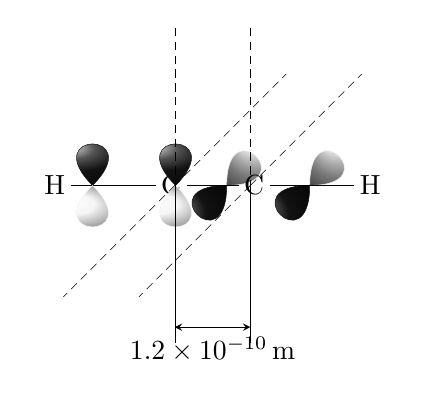
\begin{tikzpicture}[>=stealth]
  \node {
  \chemfig{
    H-[:0,1.4]C({\orbital{p}}{\orbital[angle=225]{p}})
    -C({\orbital{p}}{\orbital[angle=225]{p}})
    (-[:0,1.4]H)
    }
  };
  \draw[very thin](-0.48,0)--(-0.48,-2);
  \draw[very thin,densely dashed](-0.48,2)--(-0.48,-1)(0.48,2)--(0.48,-1);
  \draw[very thin,densely dashed](-0.48,0)--++(45:2)(-0.48,0)--++(45:-2);
  \draw[very thin,densely dashed](0.48,0)--++(45:2)(0.48,0)--++(45:-2);
  \draw[very thin](0.48,0)--(0.48,-2);
  \draw[very thin,<->](-0.48,-1.8)--(0.48,-1.8)node[midway,below]{\qty{1.2e-10}{m}};
\end{tikzpicture}
\end{document}